% =====================================================================
%  Hackathon "Embedded & KI" – Einführung: Sicherheit, Best Practices, Regeln
%  Basis: Ersti-Begrüßung-Vorlage (metropolis), Farben/Logo Fachschaft IT
%  Bauen:  pdflatex main.tex   (2x, wegen Gliederung)  oder  ./BuildTex.sh
%  Offene Stellen sind mit \TODO{...} markiert (rot im PDF, per grep findbar)
% =====================================================================
\documentclass[10pt]{beamer}

\usetheme{metropolis}
\usepackage{appendixnumberbeamer}
\usepackage{tabularx,booktabs}
\usepackage{fontawesome}
\usepackage[english,ngerman]{babel}
\graphicspath{ {./images} }
\usepackage{float,xcolor,csquotes,etoolbox}
\usepackage{listings}

\usepackage{hyperref}
\hypersetup{breaklinks,colorlinks,linkcolor=black,citecolor=black,filecolor=black,urlcolor=black}
\newcommand\urls[1]{\href{https://#1}{\nolinkurl{#1}}}

\usepackage{tikz}
\usetikzlibrary{babel,arrows.meta,positioning}
\usepackage{xspace}
\usepackage{qrcode}
\qrset{level=H,hyperlink}

% ---------------------------------------------------------------------
%  Farben Fachschaft IT
% ---------------------------------------------------------------------
\definecolor{fsitred}{HTML}{DB2F57}
\definecolor{fsitgray}{HTML}{323232}
\definecolor{fsitlight}{HTML}{F3F3F3}
\definecolor{okgreen}{HTML}{2E8B57}

\setbeamercolor{normal text}{fg=fsitgray,bg=white}
\setbeamercolor{alerted text}{fg=fsitred}
\setbeamercolor{example text}{fg=okgreen}
\setbeamercolor{frametitle}{fg=white,bg=fsitgray}
\setbeamercolor{progress bar}{fg=fsitred,bg=fsitred!20}
\setbeamercolor{title separator}{fg=fsitred}
\setbeamercolor{palette primary}{fg=white,bg=fsitgray}
\setbeamercolor{background canvas}{bg=white}
\setbeamercolor{block title}{fg=white,bg=fsitgray}
\setbeamercolor{block body}{bg=fsitlight}
\setbeamercolor{block title alerted}{fg=white,bg=fsitred}
\setbeamercolor{block body alerted}{bg=fsitred!8}
\setbeamercolor{block title example}{fg=white,bg=okgreen}
\setbeamercolor{block body example}{bg=okgreen!8}
\metroset{block=fill,progressbar=frametitle,numbering=fraction}
% Standout-Folien ("Fragen?", Merksätze) in Fachschafts-Rot
\newenvironment{redstandout}{\setbeamercolor{palette primary}{fg=white,bg=fsitred}}{}

% kleines Logo rechts in der Titelleiste
\addtobeamertemplate{frametitle}{}{%
  \begin{tikzpicture}[remember picture,overlay]
    \node[anchor=north east,inner sep=0pt] at ([xshift=-2.5mm,yshift=-1.6mm]current page.north east)
      {
\includegraphics[height=6mm]{fsit_square.pdf}};
  \end{tikzpicture}}

% ---------------------------------------------------------------------
%  Sponsoren (unten rechts) – Titel- und Endfolie
% ---------------------------------------------------------------------
\newcommand{\sponsors}{%
  \begin{tikzpicture}[remember picture,overlay]
    \node[anchor=south east,inner sep=0pt,align=right]
      at ([xshift=-5mm,yshift=4mm]current page.south east) {%
        {\scriptsize\color{fsitgray}Sponsored by}\\[1.2mm]
        
\includegraphics[height=15mm]{AstaRgb.png}\hspace{3mm}%
        
\includegraphics[height=15mm]{Logo_VF_Alumni-Friends_cube_p_rgb.png}};
  \end{tikzpicture}}
% an die Titelseite anhängen
\addtobeamertemplate{title page}{}{\sponsors}

% ---------------------------------------------------------------------
%  Helfer
% ---------------------------------------------------------------------
% Bildquelle klein unten rechts
\newcommand{\credit}[1]{\par\vfill\hfill{\tiny\color{gray}Quelle: #1}}
\newcommand{\TODO}[1]{\textcolor{fsitred}{\textbf{[TODO: #1]}}}
\newcommand{\must}{\textcolor{fsitred}{\textbf{MUSS}}\xspace}
\newcommand{\never}{\textcolor{fsitred}{\textbf{NIE}}\xspace}
\newcommand{\warn}{\item[\textcolor{fsitred}{\faWarning}]}
\newcommand{\good}{\item[\textcolor{okgreen}{\faCheck}]}
\newcommand{\bad}{\item[\textcolor{fsitred}{\faTimes}]}

\lstset{basicstyle=\ttfamily\footnotesize,columns=fullflexible,
  keywordstyle=\color{fsitred}\bfseries,commentstyle=\color{gray},
  backgroundcolor=\color{fsitlight},frame=none,xleftmargin=4pt,
  literate={ä}{{\"a}}1 {ö}{{\"o}}1 {ü}{{\"u}}1 {ß}{{\ss}}1}

% ---------------------------------------------------------------------
\title{Hackathon: Embedded \& KI}
\subtitle{Sicherheit, Best Practices \& Spielregeln}
\date{04.12.2026}
\author{Silas Mack}
\institute{Fachschaft IT}
\titlegraphic{\hfill
\includegraphics[height=1.0cm]{fsit_v1.pdf}}

\begin{document}

\maketitle

\begin{frame}{Gliederung}
  \setbeamertemplate{section in toc}[sections numbered]
  \tableofcontents[hideallsubsections]
\end{frame}

% =====================================================================
\section{Strom \& Spannung}
% =====================================================================

\begin{redstandout}
\begin{frame}[standout]
  \Huge 3,3\,V\\[0.4em]
  \large Alle unsere Boards arbeiten mit 3,3\,V Logik.\\
  5\,V an einem GPIO = Board frittiert.
\end{frame}
\end{redstandout}

\begin{frame}{Die Versorgungsspannung}
  \begin{columns}[T]
    \begin{column}{0.5\textwidth}
      \textbf{Die Pins am Board}
      \begin{itemize}
        \item \textbf{5V / VIN / VUSB}: kommt direkt vom USB.\\Nur für die Versorgung, \never an einen GPIO.
        \item \textbf{3V3}: geregelte 3,3\,V für Sensoren \& Module.
        \item \textbf{GND}: Masse, Bezugspunkt für alles.
      \end{itemize}
    \end{column}
    \begin{column}{0.5\textwidth}
      \begin{alertblock}{Vorher prüfen}
        \begin{itemize}
          \item Welche Spannung braucht das Modul?
          \item Welche Spannung gibt es an seinen \emph{Ausgängen} aus?
          \item Im Zweifel: Datenblatt lesen oder fragen.
        \end{itemize}
      \end{alertblock}
    \end{column}
  \end{columns}
  \vspace{1em}
  \begin{itemize}
    \warn GPIOs von ESP32 \emph{und} Raspberry Pi Pico sind \textbf{nicht} 5\,V-tolerant.
  \end{itemize}
\end{frame}

% Quelle: https://www.makerguides.com/wp-content/uploads/2025/04/image-154-1024x468.png
\begin{frame}{Pinout: ESP32-S3}
  \centering
  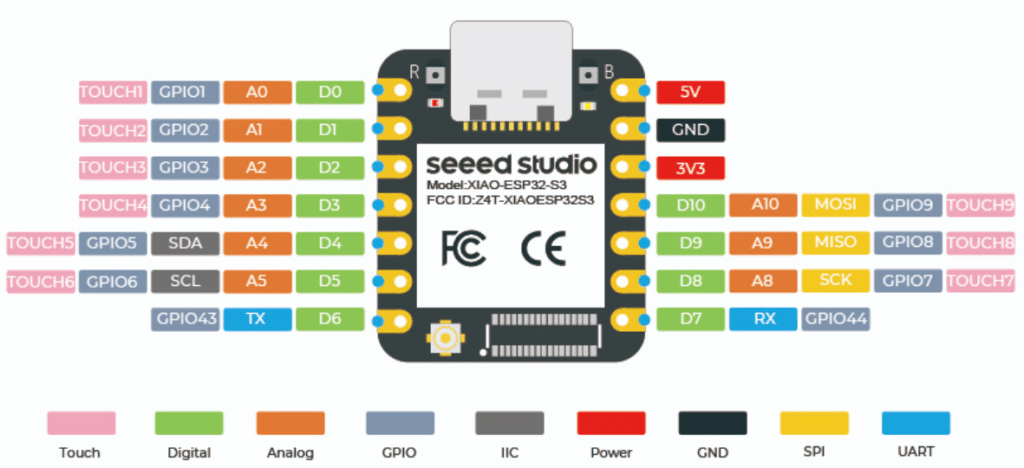
\includegraphics[width=\textwidth]{ESP32-S3_Pinout.png}
  \credit{makerguides.com}
\end{frame}

% Quelle: https://www.giga.de/ratgeber/tipps/was-bedeutet-rtfm/
\begin{frame}{Im Zweifel: Datenblatt lesen}
  \centering
  
\includegraphics[height=0.68\textheight]{RTFM-Meme.jpg}
  \credit{giga.de}
\end{frame}

\begin{frame}{Strom: Was ein Pin aushält}
  \begin{itemize}
    \item Ein GPIO ist ein \textbf{Signal}, keine Stromversorgung.\\
          ESP32: ca.\ 20\,mA pro Pin als Richtwert, Pico deutlich weniger.
    \item \textbf{LEDs} immer mit Vorwiderstand (bei 3,3\,V z.\,B.\ 220--330\,$\Omega$).
    \item \textbf{Servos, Motoren, LED-Streifen, Lautsprecher}:\\
          \never direkt am GPIO und nicht am 3V3-Pin.\\
          Eigene 5\,V-Versorgung, Steuersignal vom GPIO, GND gemeinsam.
    \item Motoren brauchen einen Treiber (Transistor / Motortreiber-Modul).
  \end{itemize}
  \vspace{0.5em}
  \begin{exampleblock}{Faustregel}
    Alles, was sich bewegt, leuchtet (mehr als eine LED) oder Krach macht,
    braucht eine eigene Versorgung.
  \end{exampleblock}
\end{frame}

% =====================================================================
\section{Verdrahten}
% =====================================================================

% Quelle: https://i1.wp.com/agoering.github.io/spice-pinball/img/learn_arduino_breadboard_edit.png?strip=all
% Bild als images/breadboard.png ablegen (konnte nicht automatisch geladen werden)
\begin{frame}{Das Steckbrett}
  \centering
  \IfFileExists{images/breadboard.png}{%
    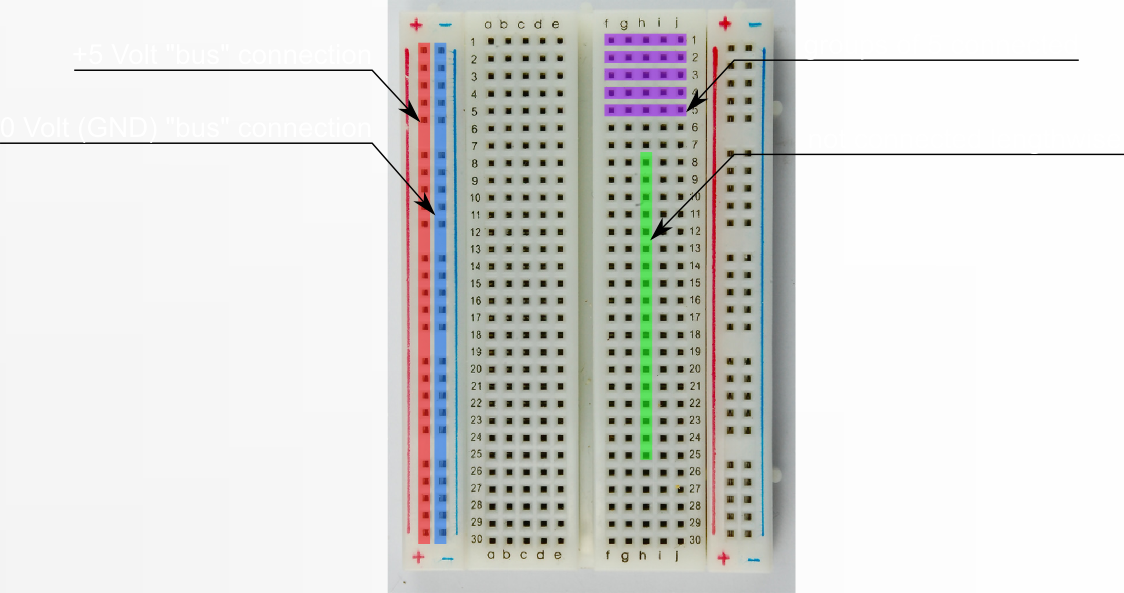
\includegraphics[height=0.72\textheight]{breadboard.png}%
  }{%
    \fbox{\parbox[c][0.6\textheight][c]{0.8\textwidth}{\centering
      \TODO{images/breadboard.png ablegen}}}%
  }
  \credit{agoering.github.io/spice-pinball}
\end{frame}

\begin{frame}{Verdrahten ohne Rauch}
  \begin{enumerate}
    \item \textbf{Stromlos} stecken: USB ab, Akku ab, dann verdrahten.
    \item \textbf{GND} gemeinsam: alle Teile, alle Netzteile.
    \item \textbf{Polarität} prüfen: \textcolor{fsitred}{rot = +}, schwarz = GND\\
          (bei Billig-Kabeln nicht blind auf die Farben verlassen).
    \item \textbf{Kurzschlüsse} vermeiden: keine Drahtreste, Schrauben oder
          Werkzeug unter dem Board.
    \item \textbf{Nochmal schauen} (oder Teamkollegen schauen lassen).
    \item Im Zweifel mit dem \textbf{Multimeter} messen.
    \item Erst dann Strom drauf.
  \end{enumerate}
\end{frame}

\begin{frame}{Wenn es heiß wird oder riecht}
  \begin{columns}[c]
    \begin{column}{0.55\textwidth}
      \begin{alertblock}{Sofort}
        \begin{enumerate}
          \item Stromversorgung trennen (USB / Akku ab)
          \item Nicht anfassen, abkühlen lassen
          \item Bescheid sagen
        \end{enumerate}
      \end{alertblock}
    \end{column}
    \begin{column}{0.42\textwidth}
      Warnzeichen:
      \begin{itemize}
        \item Chip oder Regler zu heiß zum Anfassen
        \item Brandgeruch, Rauch
        \item Laptop meldet \enquote{USB-Gerät überlastet}
      \end{itemize}
    \end{column}
  \end{columns}
  \vspace{1em}
  Kaputt ist kaputt, das ist okay. Aber bitte \textbf{melden}, damit niemand
  anderes das Teil wieder benutzt.
\end{frame}

% USB-Icon: https://www.flaticon.com/free-icons/usb-data
\begin{frame}{Handhabung \& ESD}
  \begin{columns}[c]
    \begin{column}{0.74\textwidth}
      \begin{itemize}
        \item Boards am Rand anfassen, nicht an Chips und Pins.
        \item Vorher kurz an geerdetes Metall (Heizkörper, Tischgestell) fassen.
        \item Boards nicht auf Metall, Alufolie oder in Plastiktüten ablegen.
        \item \textbf{Keine Getränke neben den Aufbau.}
        \item \textbf{USB-Kabel}: Reine Ladekabel haben keine Datenleitungen\\
              \(\Rightarrow\) Board wird nicht erkannt.
      \end{itemize}
    \end{column}
    \begin{column}{0.22\textwidth}
      \centering
      
\includegraphics[width=0.85\textwidth]{usb.png}
    \end{column}
  \end{columns}
  \credit{USB-Icon: flaticon.com}
\end{frame}

% =====================================================================
\section{Akkus}
% =====================================================================

\begin{frame}{Akkus: die Regeln}
  \begin{alertblock}{Pflicht}
    \begin{itemize}
      \item Akkus (18650, LiPo) gibt es \textbf{nur auf Anfrage}.
      \item Der \textbf{erste Anschluss} eines Akkus an eure Schaltung
            \must \textbf{außerhalb des Gebäudes} stattfinden.
      \item Laden nur über das Board, an dem der Akku hängt (LoRa-Board bzw.\ XIAO), per USB-C.
      \item Laden \never unbeaufsichtigt.
    \end{itemize}
  \end{alertblock}
  \vspace{0.3em}
  Lithium-Akkus liefern bei einem Kurzschluss sehr hohe Ströme.
  Dann wird es heiß, und im Extremfall brennt es.
  Ein Akkubrand lässt sich kaum löschen.
\end{frame}

\begin{frame}{Akkus: Umgang}
  \begin{itemize}
    \warn \textbf{Polarität} doppelt prüfen. Bei JST-Steckern von LiPos ist
          die Belegung nicht genormt!
    \warn Akku \never direkt an 3V3 oder einen GPIO (voll geladen: 4,2\,V).
          Nur an die dafür vorgesehenen Anschlüsse (z.\,B.\ BAT-Pads am XIAO).
    \warn Kein Kurzschluss: Akkus nicht lose in der Tasche, nicht auf Metall.
    \warn \textbf{Aufgeblähte}, beschädigte oder heiße Akkus nicht weiter benutzen,
          sofort melden.
  \end{itemize}
\end{frame}

% =====================================================================
\section{Löten}
% =====================================================================

\begin{frame}{Lötkolben}
  \begin{columns}[T]
    \begin{column}{0.5\textwidth}
      \begin{alertblock}{Regeln}
        \begin{itemize}
          \item Lötkolben gibt es \textbf{nur auf Anfrage}.
          \item Wer noch nie gelötet hat: nur \textbf{mit Aufsicht}.
          \item Nach Gebrauch ausschalten und zurückgeben.
        \end{itemize}
      \end{alertblock}
    \end{column}
    \begin{column}{0.47\textwidth}
      \small
      \textbf{Beim Löten}
      \begin{itemize}
        \item Die Spitze hat über 300\,°C.
        \item Auf der Spitze muss \textbf{immer Zinn} sein, auch in der Ablage.
        \item Kolben immer in die Ablage.
        \item Dritte Hand benutzen, nichts in der Hand halten.
        \item Nicht in den Rauch atmen, Fenster auf.
        \item Board ist dabei stromlos.
        \item Nach dem Löten Hände waschen.
      \end{itemize}
    \end{column}
  \end{columns}
  \vspace{0.2em}
  \small Die meisten Aufbauten gehen auch ohne Löten: Steckbrett \& Dupont-Kabel.
\end{frame}

\begin{frame}{Löten}
  \centering
  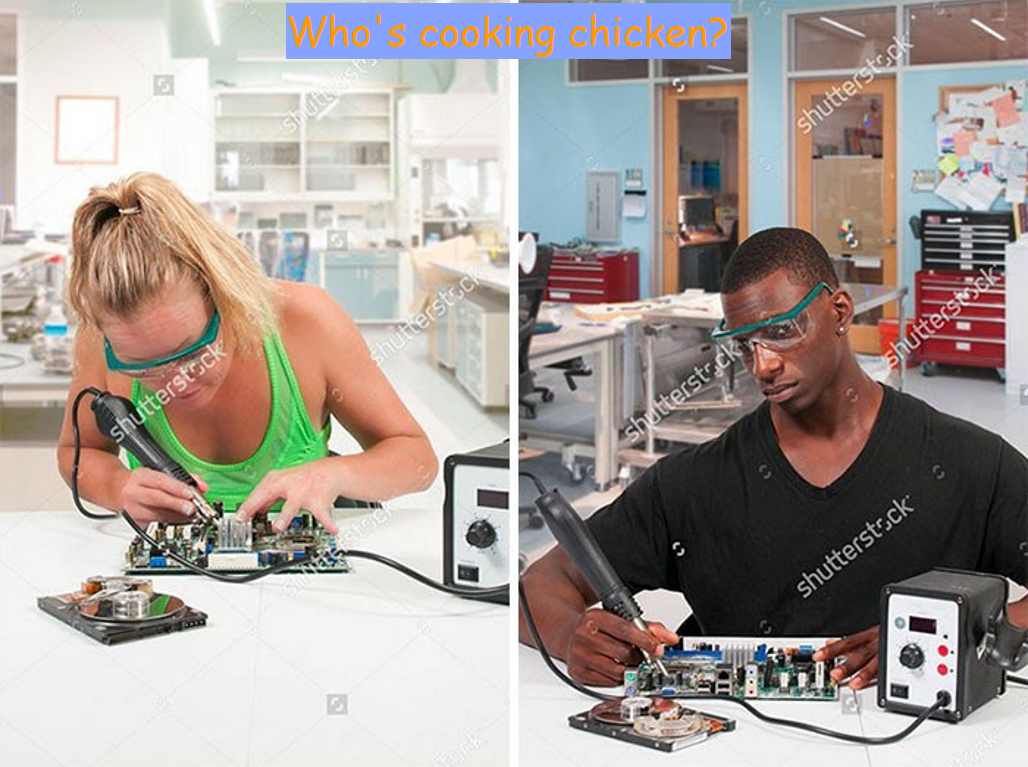
\includegraphics[height=0.75\textheight]{why_does_it_smell_like_chicken.png}
\end{frame}

% =====================================================================
\section{Material \& Ausleihe}
% =====================================================================

\begin{frame}{Material}
  \begin{itemize}
    \item Basis-Material liegt offen aus: Steckbretter, Kabel, Widerstände, LEDs, Sensoren.
    \item Boards, Module mit Wert, Akkus, Lötkolben: \textbf{über den Ausleihschein}.
    \item Nehmt nur, was ihr braucht. 20 Teams teilen sich den Pool.
    \item Kaputte Teile \textbf{nicht} zurück in die Kiste, sondern bei uns abgeben.
    \item Nach dem Event: alles Ausgeliehene vollständig zurückgeben
    \item Treff: Freitag: 11.12.2026 13-14 Uhr. Fachschaftsraum-IT
  \end{itemize}
\end{frame}

% =====================================================================
\section{Competition: Ablauf \& Regeln}
% =====================================================================

\begin{frame}{Ablauf}
  \centering
  \begin{tikzpicture}[
      phase/.style={draw=fsitgray,fill=fsitlight,rounded corners=3pt,
                   minimum width=1.85cm,minimum height=1.0cm,align=center,
                   font=\footnotesize},
      key/.style={phase,fill=fsitred,draw=fsitred,text=white,font=\footnotesize\bfseries},
      arr/.style={-{Stealth[length=2mm]},thick,fsitgray},
      node distance=0.35cm]
    \node[phase] (p) {Kurz-\\Pitch};
    \node[phase,right=of p] (z) {Zwischen-\\präsentation};
    \node[key,right=of z] (a) {Abgabe\\Eventtag};
    \node[phase,right=of a] (w) {1 Woche\\ausarbeiten};
    \node[key,right=of w] (f) {Finale\\Einreichung};
    \draw[arr] (p) -- (z); \draw[arr] (z) -- (a);
    \draw[arr] (a) -- (w); \draw[arr] (w) -- (f);
    \begin{scope}[every node/.style={font=\scriptsize,text width=1.85cm,align=center}]
      \node[below=0.2cm of p] {19-20 Uhr};
      \node[below=0.2cm of z] {~24 Uhr};
      \node[below=0.2cm of a] {05.12.};
      \node[below=0.2cm of f] {11.12.\\13-14 Uhr};      
    \end{scope}
    \draw[thick,fsitgray] ([yshift=0.4cm]p.north west) -- ([yshift=0.4cm]a.north east)
      node[midway,above,font=\footnotesize\bfseries] {Eventtag};
  \end{tikzpicture}
  \vspace{1em}

  \raggedright
  Danach bewerten wir alle Projekte.
\end{frame}

\begin{frame}{1. Kurz-Pitch}
  \begin{itemize}
    \item Jedes Team stellt seine Idee kurz vor: Maximal 3 minuten
    \item Was baut ihr? Für wen oder wofür?
    \item Welche Hardware braucht ihr ungefähr?
    \item Wo kommt KI ins Spiel?
  \end{itemize}
  \vspace{0.5em}
  \begin{exampleblock}{Ziel}
    Alle wissen, woran die anderen arbeiten. Und ihr habt euch auf eine Idee festgelegt.
  \end{exampleblock}
\end{frame}

\begin{frame}{2. Zwischenpräsentation}
  \begin{itemize}
    \item Wo steht ihr? Was läuft schon, was noch nicht?
    \item Woran hängt ihr gerade? Braucht ihr Hilfe oder Material?
    \item Plan bis zur Abgabe am Abend
    \item Dauer: Maximal 3 Minuten
  \end{itemize}
  \vspace{0.5em}
  Kein Druck: Ein halb fertiger Aufbau ist hier völlig normal.
\end{frame}

\begin{frame}{3. Abgabe am Eventtag}
  Zum Ende des Eventtags gebt ihr euren Stand ab:
  \begin{itemize}
    \item Code in eurem Team-Repo in der GitHub-Organisation\\
          {\small(bei Problemen mit GitHub: per Mail an uns)}
    \item Kurze Beschreibung: Idee, Hardware, Stand
    \item Sehr gerne Foto oder kurzes Video vom Aufbau
  \end{itemize}
  \vspace{0.5em}
  \begin{alertblock}{Wichtig}
    Nur wer am Eventtag seinen Fortschritt vorzeigt, kann in der Woche danach weitermachen und final einreichen.
  \end{alertblock}
\end{frame}

\begin{frame}{4. Eine Woche Ausarbeitung \& finale Einreichung}
  \begin{itemize}
    \item Ihr habt \textbf{eine Woche} Zeit, euer Projekt fertig zu machen.
    \item Finale Einreichung bis \textbf{11.12.2026}, 13--14 Uhr
    \item Einreichen: Hardware, Code und Doku im Team-Repo\\
          {\small(bei Problemen mit GitHub: per Mail an uns)}
  \end{itemize}
  \vspace{0.5em}
  Danach bewerten wir die Projekte final.
\end{frame}

\begin{frame}{Allgemeine Regeln}
  \begin{itemize}
    \item Teamgröße: Empfohlen sind 2 - maximal 3 Personen
    \item KI-Tools sind ausdrücklich erlaubt und erwünscht\\
          (z.\,B.\ GitHub Copilot, Google AI Studio).
    \item Fremder Code und Bibliotheken sind okay, gebt die Quellen an.
    \item Fair bleiben: Material teilen, anderen Teams helfen ist gern gesehen.
    \item Sicherheitsregeln aus dieser Präsentation gelten für alle.\\
          Wer sie ignoriert, gibt Lötkolben bzw.\ Akku zurück.
  \end{itemize}
\end{frame}

% Anmeldung zur GitHub-Organisation: Daumen hoch auf Issue #1, Einladung kommt per Skript
\begin{frame}{GitHub: Anmeldung}
  \begin{columns}[c]
    \begin{column}{0.42\textwidth}
      \centering
      \qrcode[height=4.2cm]{https://github.com/FS-IT-Hochschule-Esslingen-Hackathon/HackathonEmbedded-AI/issues}\\[0.4em]
      {\scriptsize\urls{github.com/FS-IT-Hochschule-Esslingen-Hackathon/HackathonEmbedded-AI/issues}}
    \end{column}
    \begin{column}{0.55\textwidth}
      \begin{enumerate}
        \item QR-Code scannen, mit eurem \textbf{GitHub-Account} einloggen\\
              {\small(noch keinen? \(\rightarrow\) github.com \(\rightarrow\) Sign up)}
        \item Auf dem Issue \textbf{\faThumbsUp} drücken\\
              {\small(unter dem Text auf \faSmileO{} klicken)}
        \item Einladung annehmen: Mail oder\\
              {\small\urls{github.com/orgs/FS-IT-Hochschule-Esslingen-Hackathon/invitation}}\\
              \(\rightarrow\) \textbf{Join}
      \end{enumerate}
      \vspace{0.3em}
      {\small Die Einladung kommt nicht sofort, wir verschicken sie in Runden.}
    \end{column}
  \end{columns}
\end{frame}

\begin{frame}{GitHub: Euer Team-Repo}
  \textbf{Eine Person pro Team:}
  \begin{enumerate}
    \item Oben rechts \textbf{+} \(\rightarrow\) \textbf{New repository}
    \item \textbf{Owner:} \texttt{FS-IT-Hochschule-Esslingen-Hackathon} (nicht euer eigener Account!)
    \item \textbf{Repository name:} \texttt{HackathonWS26-27\_Teamname}\\
          {\small z.\,B.\ \texttt{HackathonWS26-27\_SmartPlant}, ohne Leerzeichen}
    \item \textbf{Private}, \textbf{Add README} an \(\rightarrow\) \textbf{Create repository}
    \item \textbf{Settings} \(\rightarrow\) \textbf{Collaborators and teams} \(\rightarrow\) \textbf{Add people}\\
          \(\rightarrow\) Teammitglieder mit Rolle \textbf{Write} hinzufügen
  \end{enumerate}
\end{frame}

% Hintergrund: brennendes Steckbrett, Quelle: Bing-Bildersuche
% https://external-content.duckduckgo.com/iu/?u=https%3A%2F%2Ftse1.mm.bing.net%2Fth%2Fid%2FOIP.Mw4Hnj8uORXFsSuWppJ-XAHaFj%3Fpid%3DApi&f=1
{
  \usebackgroundtemplate{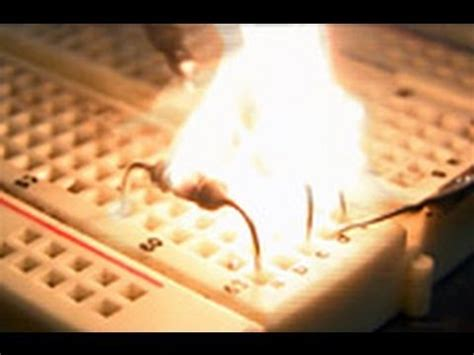
\includegraphics[width=\paperwidth,height=\paperheight]{BackgrEnd.jpg}}
  \begin{frame}[plain]
    \begin{tikzpicture}[remember picture,overlay]
      \node[fill=black,fill opacity=0.55,text opacity=1,text=white,
            inner xsep=1.2em,inner ysep=0.6em,rounded corners=4pt,
            font=\Huge\bfseries] at (current page.center) {Fragen?};
    \end{tikzpicture}
  \end{frame}
}

% Endfolie mit Sponsoren
\begin{frame}[plain]
  \centering
  \vfill
  {\Huge\bfseries\color{fsitgray}Danke \& viel Spaß!}\\[1em]
  {\large\color{fsitred}Hackathon: Embedded \& KI}
  \vfill
  \begin{tikzpicture}[remember picture,overlay]
    \node[anchor=south west,inner sep=0pt]
      at ([xshift=5mm,yshift=4mm]current page.south west)
      {
\includegraphics[height=8mm]{fsit_v1.pdf}};
  \end{tikzpicture}%
  \sponsors
\end{frame}

\end{document}
